\subsection{Beyond relational queries}

\dbsp can express programs that go beyond Datalog, SQL, or incremental
versions of these: see the non-monotonic semantics for Datalog$^\neg$
and Datalog$^{\neg\neg}$\cite{Abiteboul-book95}.  \dbsp can model many
classes of streaming operators and stateful streaming computations.

For example, to illustrate the Turing-completeness of \dbsp, we
implement the following \emph{while} program, where $Q$ is an
arbitrary query: {\small
\begin{lstlisting}[language=Pascal]
x := i;
while (x changes)
    x := Q(x);
\end{lstlisting}}
The \dbsp implementation of this program is:

%$$\lambda i. \int[\D[\fix{\xi}{Q(\delta(i)+\zm(\xi))}]]$$
\begin{center}
\begin{tikzpicture}[>=latex]
  \node[] (input) {$i$};
  \node[block, right of=input] (delta) {$\delta$};
  \node[block, circle, right of=delta, inner sep=0cm] (p) {$+$};
  \node[block, right of=p] (Q) {$\lift Q$};
  \node[block, right of=Q] (D) {$\D$};
  \node[block, right of=D] (S) {$\int$};
  \node[right of=S] (output)  {$x$};
  \node[block, below of=p, node distance=.8cm] (z) {$\zm$};
  \draw[->] (input) -- (delta);
  \draw[->>] (delta) -- (p);
  \draw[->>] (p) -- (Q);
  \draw[->>] (Q) -- node (mid) {} (D);
  \draw[->>] (D) -- (S);
  \draw[->>] (mid.center) |- (z);
  \draw[->] (S) -- (output);
  \draw[->>] (z) -- (p);
\end{tikzpicture}
\end{center}

This circuit can be converted to a streaming circuit that computes a stream of values $i$
by lifting it; it can be incrementalized using Algorithm~\ref{algorithm-inc} to compute on changes of $i$:

\noindent
\begin{center}
\begin{tikzpicture}[>=latex]
  \node[] (input) {$\Delta i$};
  \node[block, right of=input] (delta) {$\lift{\delta}$};
  \node[block, circle, right of=delta, inner sep=0cm] (p) {$+$};
  \node[block, right of=p, node distance=1.3cm] (Q) {$\inc{(\lift{\lift{Q}})}$};
  \node[block, right of=Q, node distance=1.5cm] (D) {$\lift{\D}$};
  \node[block, right of=D, node distance=1.1cm] (S) {$\lift{\int}$};
  \node[right of=S, node distance=1.2cm] (output)  {$\Delta x$};
  \node[block, below of=p, node distance=.9cm] (z) {$\lift{\zm}$};
  \draw[->>] (input) -- (delta);
  \draw[->>>] (delta) -- (p);
  \draw[->>>] (p) -- (Q);
  \draw[->>>] (Q) -- node (mid) {} (D);
  \draw[->>>] (D) -- (S);
  \draw[->>>] (mid.center) |- (z);
  \draw[->>] (S) -- (output);
  \draw[->>>] (z) -- (p);
\end{tikzpicture}
\end{center}

At runtime the execution of this circuit is not guaranteed to terminate;
however, if the circuit does terminate, it will produce the correct
output, i.e., the least fixpoint of $Q$ that includes~$i$.

\section{Implementation}\label{sec:implementation}

In this section we describe an implementation of a SQL compiler and
runtime that targets DBSP.  Figure~\ref{fig:tools} shows the compiler
structure.

\begin{figure}[h]
  \begin{center}
    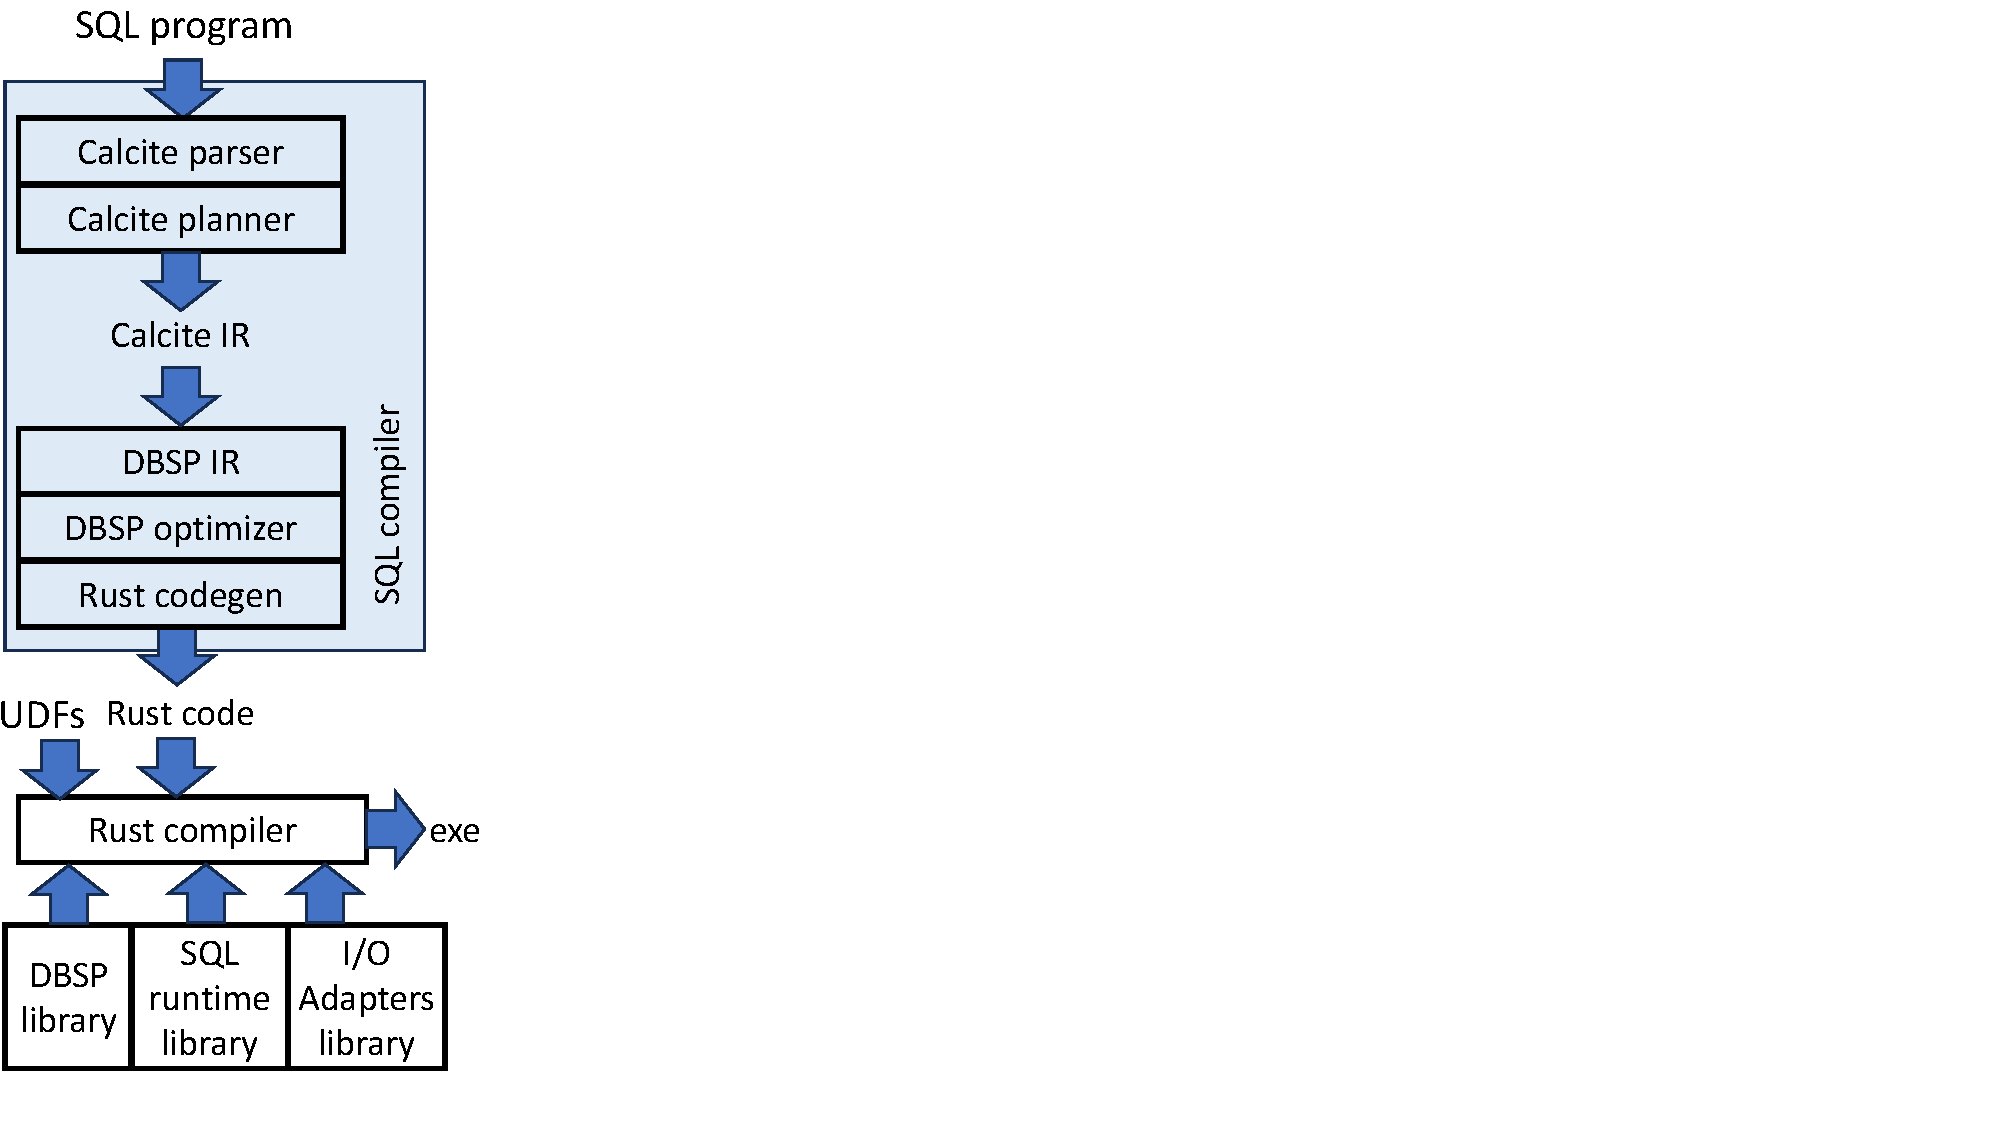
\includegraphics[trim={0 0in 10in 0},clip,scale=.45]{tools.pdf}
    \caption{\label{fig:tools}Architecture of the SQL compiler.}
  \end{center}
\end{figure}

\subsection{Supporting SQL}

In \secref{sec:relational} we have shown how to implement the
relational algebra using \dbsp.  However, the SQL language is
significantly richer than the relational algebra.

\paragraph{Multisets.} SQL operates on \emph{multisets} (or bags), e.g.,
\code{UNION ALL}.  Since \zrs generalize bags, they can model all SQL
operations. Many queries on multisets can be implemented by just
omitting $\distinct$ operators.

\paragraph{NULLs.} \dbsp says nothing about the data types
and the functions that are executed by the operators in each node.  In
our Rust SQL runtime (described in Section~\refsec{sec:runtime})
nullable types are represented using Rust \texttt{Option<>} types, and
SQL \code{NULL} is the value \code{None}.  Some care is required in
implementing the unusual semantics of \code{NULL} (e.g., in SQL two
\code{NULL} values are neither equal, nor different).

\paragraph{Primary keys.} A primary key changes a table's behavior on insertion:
inserting a tuple can cause another tuple to be deleted.  This
behavior looks roughly like a modified $\distinct$ operator, and can
be implemented incrementally similarly:

\begin{center}
\begin{tikzpicture}[>=latex]
    \node[] (input) {$\Delta d$};
    \node[block, right of=input] (I) {$\I$};
    \node[block, right of=I] (z) {$\zm$};
    \node[block, below of=z, node distance=.8cm] (H) {\texttt{UPSERT}};
    \node[right of=H, node distance=1.3cm] (output) {$\Delta o$};
    \draw[->>] (input) -- node (mid) {} (I);
    \draw[->>] (I) -- (z);
    \draw[->>] (mid.center) |- (H);
    \draw[->>] (z) -- node (i) [right] {} (H);
    \draw[->>] (H) -- (output);
\end{tikzpicture}
\end{center}

\noindent The \code{UPSERT} operator and converts a \zr describing an
insertion with key $k$: $\{ (k, v) \mapsto 1 \}$ to a \zr $\{ (k, v)
\mapsto 1, (k, v') \mapsto -1 \}$, where $(k, v')$ is the previous
value of the record, obtained from the $\I$ operator.

\paragraph{Constant values.}  One can write in SQL queries that have
constant outputs, e.g., \code{SELECT 2}.  Technically an operator that
produces a constant result is not TI.  However, constants can be
accommodated easily by modeling them mathematically as constant input
streams.

\subsubsection{Grouping and indexed \zrs}\label{sec:grouping}

Let $K$ be a set of ``key'' values.  The finite maps from $K$ to \zrs
are functions $K \to \Z[A] = \Z[A][K]$.  We call values $i$ of this
type \defined{indexed \zrs}: for each key $k \in K$, $i[k]$ is a \zr.
Because the codomain $\Z[A]$ is an Abelian group, this structure is
itself an Abelian group.  Here is an example indexed \zr:

\begin{center}
  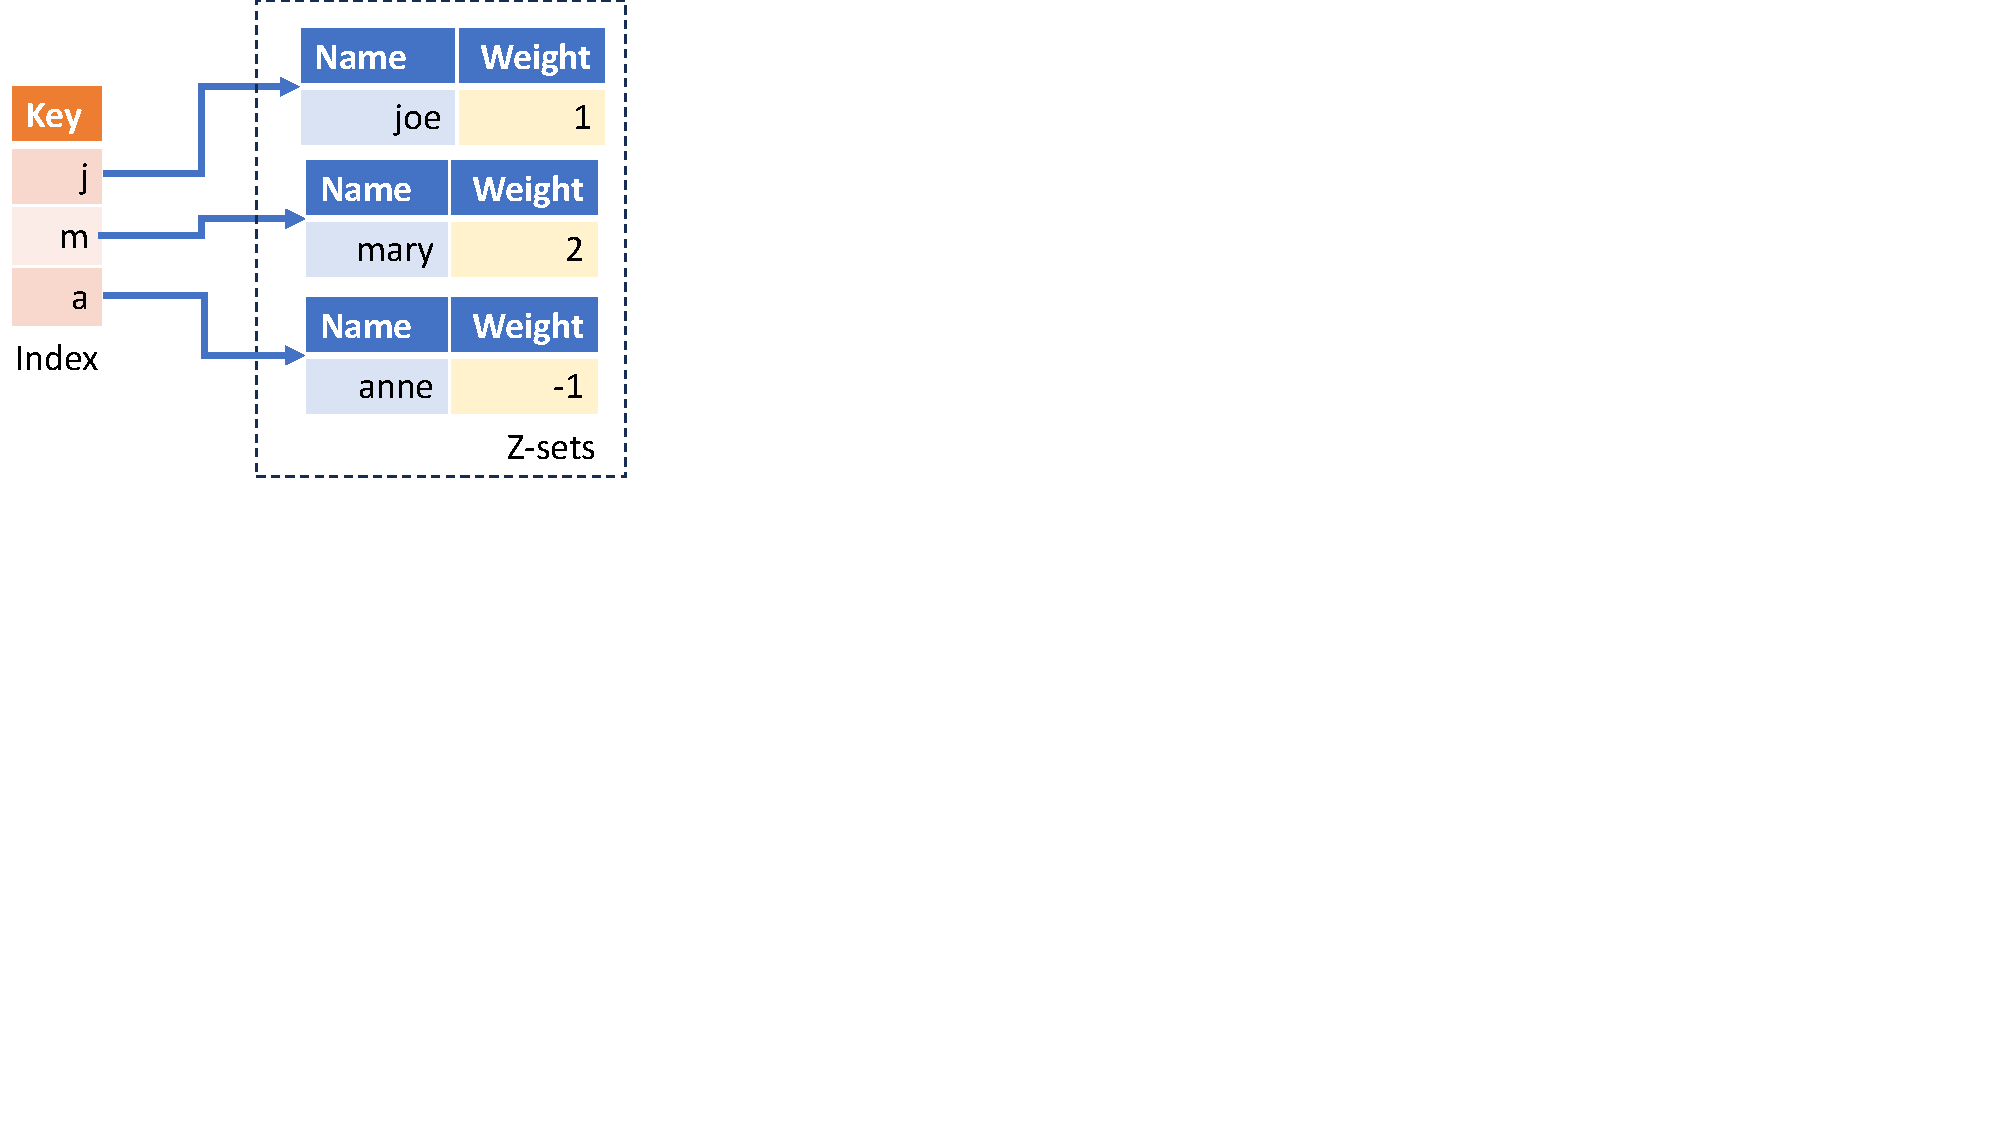
\includegraphics[trim={0 4.2in 7.5in 0},clip,scale=.34]{indexed.pdf}
\end{center}

This structure is used to implement the SQL \texttt{GROUP BY} operator
in \dbsp.  Consider a \defined{partitioning function} $p: A \to K$
that assigns a key to any value in $A$.  We define the grouping
function $G_p: \Z[A] \to \Z[A][K]$ as $G_p(a)[k] \defn \sum_{x \in
  a.p(x)=k}\{ x \mapsto a[x] \}$ (just map each element of the input
$a$ to the \zr grouping corresponding to its key).  When applied to a
\zr this function returns an indexed \zr: each key $k$ maps to a \zr
containing all elements of the group (as in SQL, each group is a
multiset).  Consider our example \zr $R$ from \refsec{sec:relational},
and a key function $p(s)$ that returns the first letter of the string
$s$.  The resulting indexed \zr is shown in the previous diagram.

The operation building an indexed \zr from a \zr is linear for any key
function!  It follows that group-by is incremental: each row changed
in the input relation produces a row changed in a group, obtained by
applying the partitioning function.

Notice that, unlike SQL, \dbsp can express naturally computations on
indexed \zrs, they are just an instance of a group structure.  In
\dbsp one does not need to follow grouping by aggregation, and \dbsp
can represent nested groupings of arbitrary depth.  Indeed, our
compiler can recognize classes of such computations expressed using
SQL windows (e.g., TopK for each group), and can generate efficient
incremental code.

%Please note that our definition of incremental computation is only
%concerned with incrementality in the \emph{outermost} structures.  We
%leave it to future work to explore an appropriate definition of
%incremental computation on the \emph{inner} relations.

\subsubsection{\texttt{UNNEST} (flatmap)}

A useful operation on nested relations is \defined{flatmap} (or
\code{UNNEST} in SQL), which one can view as the inverse of grouping,
converting an indexed \zr into a \zr.  This operation is also a linear
\dbsp operator.

\subsubsection{Aggregation}\label{sec:aggregation}

Aggregation in SQL applies a function $a$ to a set of values of type
$A$ producing a ``scalar'' result with some result type $B$.  In \dbsp
an aggregation function has a signature $a: \Z[A] \to B$.  When
operating on \zrs, aggregation functions have to multiply the
contribution of each value by its associated weight.
(\texttt{DISTINCT} aggregates have to first apply a \texttt{DISTINCT}
operator.)

Distributive (e.g. \code{SUM}) and some algebraic aggregation
(\code{AVG}) functions map can be implemented by a pair of linear
functions between \zrs and the target group: the actual aggregation
and the post-processing (e.g., dividing the sum by the counter for
average).  So apparently they are purely incremental.

The subtle point is that in SQL the result of these aggregation must
be a (singleton) set containing an element of $B$, and not a value
with type $B$.  So additional machinery is needed to convert the
values of $B$ into values of $\Z[B]$, and this transformation is
\emph{not} linear.  Consider the following query: \code{SELECT
  COUNT(*) FROM I}.  The lifted incremental version of this query is
the following circuit, where $a_\texttt{COUNT}$ is the linear
``count'' aggregation function, which just sums up the weights of the
input values:

\begin{tikzpicture}[>=latex, node distance=1.2cm]
  \node[] (in) {$\Delta$\code{I}};
  \node[block, right of=in] (pi) {$\pi_\texttt{C}$};
  \node[block, right of=pi] (a) {$a_\texttt{COUNT}$};
  \node[block, right of=a] (inc) {$\mathit{inc}$};
  \node[block, below of=inc, node distance=.7cm] (IN) {$\I$};

  \node[block, right of=inc] (I) {$\I$};
  \node[block, right of=I] (z) {$\zm$};
  \node[block, below of=z, node distance=.8cm] (H) {\texttt{UPSERT}};
  \node[right of=H, node distance=1.3cm] (output) {$\Delta o$};
  \draw[->>] (in) -- (pi);
  \draw[->>] (pi) -- (a);
  \draw[->>] (a) |- (IN);
  \draw[->>] (IN) -- (inc);
  \draw[->>] (a) -- (inc);
  \draw[->>] (I) -- (z);
  \draw[->>] (z) -- (H);
  \draw[->>] (H) -- (output);
  \draw[->>] (inc) -- node (mm) {} (I);
  \draw[->>] (mm.center) |- (H);
\end{tikzpicture}

Let's say the input table \code{I} has 2 elements, and thus the
previous aggregation result was 2.  When adding a new row, the
$\mathit{inc}$ increments the previous aggregation result (obtained
from $\I$) result with the current increment, and then the
\code{UPSERT} converts the insertion of the tuple $\{3 \mapsto 1\}$
into the \zr $\{3 \mapsto 1, 2 \mapsto -1 \}$, since the output set no
longer contains the value 2.  The $\mathit{inc}$, $\I$ and $\makeset$
operators only do work proportional to the size of the change, and
they only store $O(1)$ state.

%An aggregation function such as \texttt{AVG} can be written as the composition of
%a linear function that computes a pair of values using
%\texttt{SUM} and \texttt{COUNT}, followed by a division and a call to \makeset.

%\begin{lstlisting}[language=SQL]
%SELECT AVG(c) FROM I
%\end{lstlisting}
%
%\begin{tikzpicture}[auto,>=latex]
%  \node[] (I) {\code{I}};
%  \node[block, right of=I] (pi) {$\pi_\texttt{C}$};
%  \node[block, right of=pi, node distance=1.4cm] (sc) {$(a_\texttt{SUM}, a_\texttt{COUNT})$};
%  \draw[->] (I) -- (pi);
%  \draw[->] (pi) -- (sc);
%  \node[block, right of=sc, node distance=1.8cm] (m) {$\makeset$};
%  \node[block, right of=m, node distance=1.2cm] (div) {$\sigma_/$};
%  \node[right of=div] (O) {\code{O}};
%  \draw[->] (sc) -- (m);
%  \draw[->] (m) -- (div);
%  \draw[->] (div) -- (O);
%\end{tikzpicture}

Aggregate functions, such as \code{MIN}, are \emph{not} linear in the
presence of deletions.  The incremental form of such aggregates needs
to maintain the entire input collection, using an $\I$ operator,
similar to the $\distinct$ operator.  They can be implemented
efficiently by keeping the data organized as a priority heap sorted by
the value compared.

In SQL, \code{NULL} values do not participate in aggregation, so one
needs two insert two extra operators for collections of nullable
values:
\begin{itemize}
  \item an operator that counts the number of rows aggregated (as
    described by Mumick~\cite{mumick-sigmod97}), which is used to
    detect empty groups
  \item a filtering operator (linear), which eliminates \code{NULL}s
    prior to aggregation
\end{itemize}

For many SQL aggregation functions aggregating over an empty set
should produce a \code{NULL} result.  All aggregation circuits
described so far will return an empty \zr for an empty input.  Let $z$
be the result expected for the empty input (e.g., \code{NULL}).  The
following circuit, applied after aggregation, will produce the result
expected by SQL:

\begin{center}
\begin{tikzpicture}[auto,>=latex]
  \node[] (agg) {\code{agg}};
  \node[right of=agg] (dummy) {};
  \node[block, above of=dummy, node distance=.7cm] (map) {$\code{map}(\lambda x . z)$};
  \node[block, right of=map, shape=circle, inner sep=0in, node distance=1.5cm] (minus) {$-$};
  \node[block, below of=minus, node distance=1.4cm] (zero) {$z$};
  \node[block, right of=agg, node distance=3cm, shape=circle, inner sep=0in] (plus) {$+$};
  \node[right of=plus] (out) {$out$};
  \draw[->] (agg) -- (map);
  \draw[->] (map) -- (minus);
  \draw[->] (minus) -- (plus);
  \draw[->] (zero) -- (plus);
  \draw[->] (agg) -- (plus);
  \draw[->] (plus) -- (out);
\end{tikzpicture}
\end{center}

\noindent When \code{agg} is the empty \zr, the ``map'' node produces
an empty \zr, and the final result is just $z$.  When \code{agg} is
non-empty, the top and bottom branches of the adder cancel each other,
and the result is \code{agg}.  This scheme is also implemented by
Materialize Inc.'s IVM engine.

\subsubsection{\texttt{GROUP BY-AGGREGATE}}

Grouping in SQL is always followed by aggregation.  This can be
modeled by the composition of our solutions for grouping and
aggregation described above.  In this case, the \code{UPSERT} operator
indexes data using the group key.  For linear aggregates this operator
needs to maintain state proportional to the number of groups.  For
non-linear aggregates this maintains state proportional to the entire
input collection.

%If we use an aggregation function $a: K \times Z[A]$ that is linear in its
%second argument, then the aggregation operator $Agg_a$ is linear, and
%thus fully incremental.  As a consequence, $\mbox{flatmap}$ is linear.
%However, many practical aggregation functions for nested relations are in fact
%not linear; an example is the $count$ function above, which is not linear
%since it uses the $\makeset$ non-linear function.  Nevertheless, while
%the incremental evaluation of such functions is not fully incremental,
%it is at least partly incremental: when applying a change to groupings, the aggregation
%function only needs to be re-evaluated \emph{for groupings that have changed}.

%\subsection{Antijoin}\label{sec:antijoin}\index{antijoin}
%
%Antijoins arise in the implementation of Datalog programs with stratified negation.
%Consider the following program:
%
%\begin{lstlisting}[language=ddlog,basicstyle=\small]
%O(v, z) :- I1(v, z), not I2(v).
%\end{lstlisting}
%
%The semantics of such a rule is defined in terms of joins and set difference.
%This rule is equivalent with the following pair of rules:
%
%\begin{lstlisting}[language=ddlog,basicstyle=\small]
%C(v, z) :- I1(v, z), I2(v).
%O(v, z) :- I1(v, z), not C(v, z).
%\end{lstlisting}
%
%This transformation reduces an antijoin to a join
%followed by a set difference.  This produces the following \dbsp circuit:
%
%\begin{tikzpicture}[auto,>=latex]
%  \node[] (i1) {\code{I1}};
%  \node[below of=i1, node distance=.5cm] (i2) {\code{I2}};
%  \node[block, right of=i1, node distance=1.5cm] (join) {$\bowtie$};
%  \node[block, shape=circle, inner sep=0in, right of=join] (m) {---};
%  \node[block, above of=m, shape=circle, inner sep=0in, node distance=.6cm] (plus) {$+$};
%  \node[block, right of=plus, node distance=1cm] (distinct) {$\distinct$};
%  \node[right of=distinct, node distance=1cm] (output) {\code{O}};
%  \draw[->] (i1) -- node (tap) {} (join);
%  \draw[->] (i2) -| (join);
%  \draw[->] (join) -- (m);
%  \draw[->] (m) -- (plus);
%  \draw[->] (tap.south) |- (plus);
%  \draw[->] (plus) -- (distinct);
%  \draw[->] (distinct) -- (output);
%\end{tikzpicture}
%

\subsubsection{Other operations on SQL groups}

SQL constructs such as \code{PARTITION BY/OVER} make it possible to
write queries over groups, e.g., TOP-K.  These can be implemented in
\dbsp naturally as functions over indexed \zrs.

\begin{comment}
\subsection{Streaming joins}

Consider a binary query $T(s, t) = \I(s)~~\lift{\bowtie}~~t$.  This is the
\emph{relation-to-stream join} operator supported by streaming databases like Kafka's ksqlDB~\cite{jafarpour-edbt19}.
Stream $s$ carries changes to a relation, while $t$ carries arbitrary data, e.g., logs
or telemetry data points. $T$ discards values from $t$ after matching them against the accumulated contents of the relation $\I(s)$.

%\item[Explicit delay:]
%So far the $\zm$ operator was only used in integration or
%differentiation.  However, it can be exposed as a primitive operation that
%can be applied to streams.  This enables programs that can
%perform convolutions and time-based window computations over streams:

\paragraph{Streaming Window queries.}

Streaming databases often organize the contents of streams into windows,
which store a subset of data points with a predefined range of timestamps.
%% The circuit below computes a \emph{fixed-size sliding-window aggregate}
%% over the last four timestamps with aggregations defined by the $T_i$ functions.
%%
%% \begin{center}
%% \begin{tikzpicture}[>=latex]
%%     \node[] (input) {$s$};
%%     \node[block, right of=input, node distance=1.5cm] (f0) {$T_0$};
%%     \node[below of=input, node distance=.5cm] (fake) {};
%%     \node[block, right of=fake, node distance=1cm] (z0) {$\zm$};
%%     \node[right of=input, node distance=.35cm] (tap) {};
%%     \node[block, right of=f0, node distance=1.5cm] (f1) {$T_1$};
%%     \node[block, right of=z0, node distance=1.2cm] (z1) {$\zm$};
%%     \node[block, right of=f1, node distance=1.5cm] (f2) {$T_2$};
%%     \node[block, right of=z1, node distance=1.5cm] (z2) {$\zm$};
%%     \draw[->] (input) -- (f0);
%%     \draw[->] (tap.center) |- (z0);
%%     \draw[->] (z0) -| (f0);
%%     \draw[->] (f0) -- (f1);
%%     \draw[->] (z0) -- (z1);
%%     \draw[->] (z1) -| (f1);
%%     \draw[->] (f1) -- (f2);
%%     \draw[->] (z1) -- (z2);
%%     \draw[->] (z2) -| (f2);
%%     \node[right of=f2] (output) {$o$};
%%     \draw[->] (f2) -- (output);
%% \end{tikzpicture}
%% \end{center}
%%
In practice, windowing is usually based on physical timestamps attached to
stream values rather than logical (transaction) time as in the previous circuit.
For instance, the CQL~\cite{arasu-tr02} query
``\texttt{SELECT * FROM events [RANGE 1 hour]}'' returns all events received
within the last hour.  The corresponding circuit (on the left)
takes input stream $s \in \stream{\Z[A]}$ and an additional
input $\theta \in \stream{\mathbb{R}}$ that carries the value of the current
time.

\begin{tabular}{m{3cm}m{0.5cm}m{3cm}}
\begin{tikzpicture}[>=latex]
    \node[] (input) {$s$};
    \node[above of=input, node distance=.5cm] (t) {$\theta$};
    \node[block, right of=input] (i) {$I$};
    \node[block, right of=i] (w) {$W$};
    \node[right of=w] (output) {$o$};
    \draw[->] (input) -- (i);
    \draw[->] (i) -- (w);
    \draw[->] (w) -- (output);
    \draw[->] (t) -| (w);
\end{tikzpicture}
&
$\cong$
&
\begin{tikzpicture}[>=latex]
    \node[] (input) {$s$};
    \node[above of=input, node distance=.5cm] (t) {$\theta$};
    \node[block, shape=circle, right of=input, inner sep=0pt] (plus) {$+$};
    \node[block, right of=plus] (w) {$W$};
    \node[right of=w] (output) {$o$};
    \node[block, below of=plus, node distance=.6cm] (z) {$\zm$};
    \draw[->] (input) -- (plus);
    \draw[->] (plus) -- (w);
    \draw[->] (t) -| (w);
    \draw[->] (w) -- node (mid) {} (output);
    \draw[->] (mid.center) |-  (z);
    \draw[->] (z) -- (plus);
\end{tikzpicture} \\
\end{tabular}

\noindent{}where the \emph{window operator} $W$ prunes input \zrs, only keeping values
with timestamps less than an hour behind $\theta[t]$.  Assuming $ts: A \to \mathbb{R}$ returns
the physical timestamp of a value, $W$ is defined as $W(v, \theta)[t] \defn \{x \in v[t] .
ts(x) \geq \theta[t] - 1hr\}$.  Assuming $\theta$ increases monotonically, $W$
can be moved inside integration, resulting in the circuit on the right, which uses
bounded memory to compute a window of an unbounded stream.
This circuit is a building block of a large family of window queries, including
window joins and window aggregation (e.g., SQL \texttt{OVER} queries).

\item[Weakening assumptions]

The theory as presented requires streams to be over group elements.  However,
this is necessary only if we want to automatically compute incremental
versions of the operators --- the addition and negation operations are
required for building $\I$ and $\D$.  The streaming circuits model
works very well on much simpler algebraic structures.  The $0$ element
is still needed to define $\zm$ and time-invariance.  Circuits that
mix streams over groups with arbitrary streams are well-defined.  However,
the zero-preservation property is required even for such general computations,
for the time-invariance of the resulting circuits.
\end{comment}

\subsection{Formal verification}

We have formalized and verified all the definitions, lemmas,
propositions, theorems, and examples in this paper using the Lean
theorem prover; we make these proofs available at~\cite{dbsp-theory}.
The formalization builds on mathlib~\cite{mathlib2020}, which provides
support for groups and functions with finite support (modeling
\zrs). We believe the simplicity of \dbsp enabled completing these
proofs in relatively few lines of Lean code (5K) and keeping a close
correspondence between the paper proofs in~\cite{tr} and Lean.  The
existence of the proofs bolsters our confidence in the correctness of
our implementation.

\subsection{The \dbsp Rust runtime}\label{sec:runtime}

We have built an implementation of \dbsp as part of an
open-source~\cite{dbsp-repo} project with an MIT
license~\cite{dbsp-crate}.  The implementation consists of a Rust
library for building circuits and a runtime that executes these
circuits using a pool of worker threads.

The library provides APIs for basic algebraic data types: such as
groups, finite maps, \zrs, indexed \zrs.  The core data structure of
the library for representing data processed is the ``time-indexed,
indexed \zr''.  This is the most general data structure needed in
recursive circuits.  It represents a vector (indexed by time) of
indexed \zrs.  Simple indexed \zrs are represented by a vector with a
single element, while \zrs are represented as indexed \zrs with an
empty value.\footnote{Rust is very efficient at eliding empty data
structures.}  The starting point of this implementation was the
differential dataflow trace data structure~\cite{dd-crate}.

A circuit construction API allows users to create \dbsp circuits by
inserting operator nodes --- boxes in our diagrams --- and connecting
them with streams --- the arrows in our diagrams.  The library
provides more than 70 pre-built generic operators for integration,
differentiation, delay, nested integration and differentiation, and
basic \zr incremental operators, corresponding to plus, negation,
grouping, joining, semi-joins, anti-joins, temporal joins, primitive
aggregates, generic aggregates (fold), $\distinct$, flatmap, window
aggregates, indexing, upsert, etc.  Some operators only exist in an
pure incremental form (e.g., they only operate correctly when fed
deltas), and thus, when used in a non-incremental circuit, have to be
``inverted'' using the inversion property from
Proposition~\ref{prop-inc-properties}.

For iterative computations the library provides the $\delta$ operator
and an operator that generalizes $\int$ by terminating iteration when
all the operators in the corresponding circuit cycle have reached a
fixed point.  The low level library allows users to construct
incremental circuits manually by stitching together incremental and
non-incremental versions of primitive operators.

The library also provides many ``helper'' operators that are used by
the code generator in the implementation of some streaming queries,
e.g., for state garbage-collection (a subject not discussed in this
paper).

\subsubsection{Parallelization and Scale-out}

Besides computing on streams, \dbsp circuit look very much like other
dataflow query engines.  As such, all standard parallelization
algorithms described in the literature~\cite{Graefe-sigmod90} can be
applied.  Our core circuits library automatically parallelizes each
circuit by sharding each operators to execute using a specified number
of worker threads (all operators use the same number of threads, which
is statically-defined).  The library automatically inserts exchange
operators to re-shard data when necessary (e.g., shard on the common
key in an equi-join).  The same scheme can be used to implement
scale-out solutions across multiple machines, but this part of the
runtime is still under development.

\subsubsection{State management}\label{sec:state-management}

Incremental computation is not free.  It is in fact a trade-off
between time and space.  While many incremental query primitives are
``stateless'', some important classes of database operations,
including joins, $\distinct$, and group-by-aggregate use $\I$
operators in their incremental expansion.  This state is kept in
\emph{indexes} (called ``arrangements'' in~\cite{mcsherry-vldb20}).
(In the \dbsp theoretical model the state is stored in fact in delay
operators $\zm$ and $\lift{\zm}$, but these are always inside
integrators $\I$.)  All other operators are stateless.

The size of these indexes is proportional to the size of the total
input data of these operators --- and thus the total state of a
circuit can even exceed the size of the original database.  (Many
traditional IVM schemes opt to recompute this state on demand, rather
than store it permanently; \dbsp can model this strategy.)

At runtime, linear operators are essentially free.  The performance of
a \dbsp program is given by the cost of maintaining and
accessing the indexes.

Indexes provide two essential operations:
\begin{itemize}
\item Merging an existing (large) index with a new (small) change.
\item Looking up a (small) set of values.
\end{itemize}

Our implementation of indexes performs both these operations in
amortized time $O(k \log n)$, where $k$ is the size of the changes,
and $n$ is the size of the index.  The implementation of indexes is
essentially a Log-Structured Merge (LSM) Tree~\cite{oneil-ai96}.

The data structure used for indexes, (called a \emph{trace} in the
code), is shown in Figure~\ref{fig:trace}.  Each index is represented
as a sequence of sorted immutable lists (called \emph{batches}), of
exponentially increasing sizes (1, 2, 4, 8, etc.) --- a generalization
of binary signed digits~\cite{signed-digits}.  Any batch is sorted
lexicographically, first on the index, then on the value.  Each batch
is a \zr, and a trace represents the \zr that is the sum of all
component batches.  The same tuple can appear in different batches
with different weights, but appears at most once in each batch.  Since
addition is commutative and associative, parts can be added in any
order.

\begin{figure}[h]
  \begin{center}
    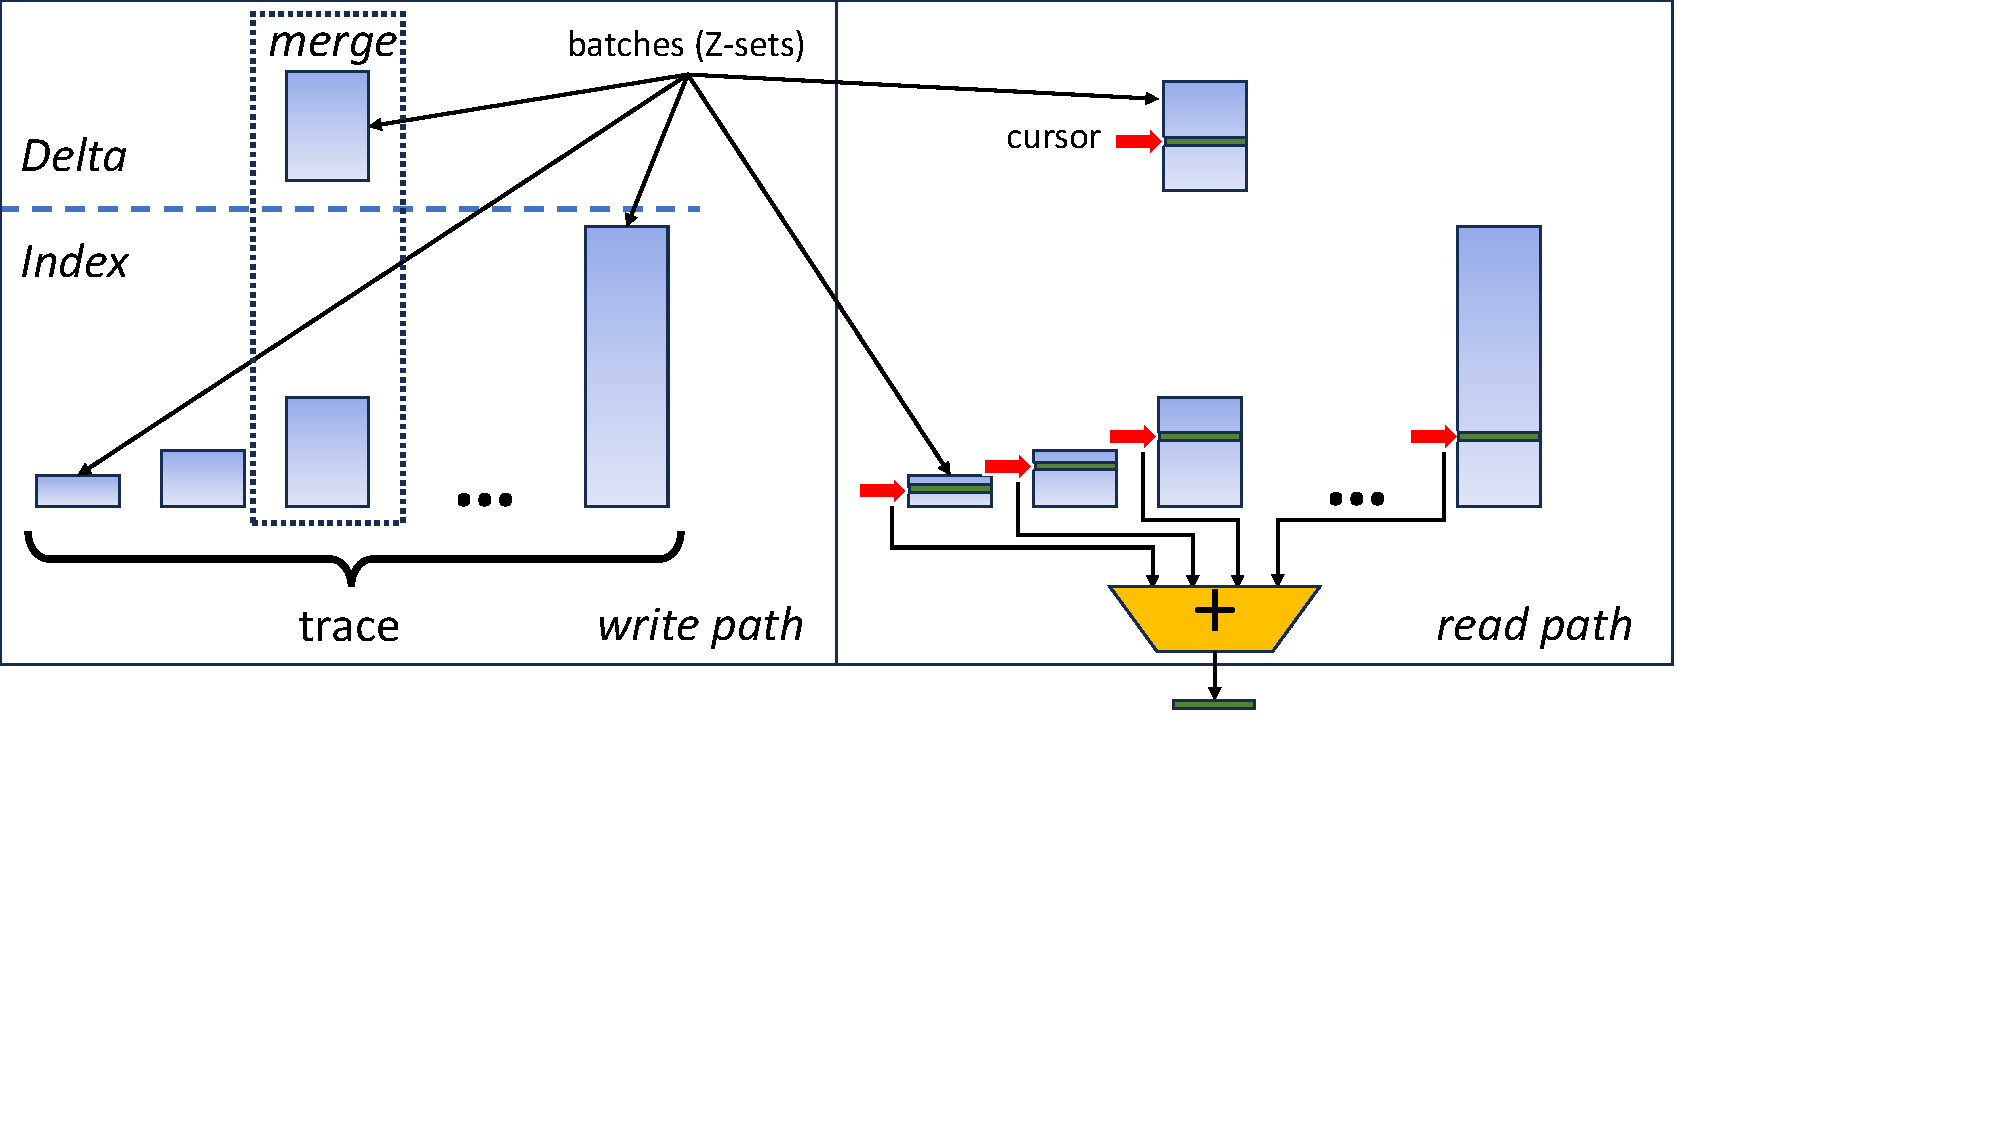
\includegraphics[trim={0 2.9in 2.1in 0},clip,scale=.27]{trace.pdf}
    \caption{\label{fig:trace}Index representation and access.}
  \end{center}
\end{figure}

A change added to an index is represented as a single batch, sorted
using the same order as the index.  When the index ingests a new
change (left side of Figure~\ref{fig:trace}), the new batch is simply
appended.  As the index grows, batches of similar size are lazily
merged.  A merge may require multiple circuit steps.  The result of
merging 2 batches with \(n_1\) and \(n_2\) tuples has \(n_1 +
n_2\) or fewer tuples, and can even be empty if all weights add to 0.

To lookup the tuples of a change inside an index (right side of
Figure~\ref{fig:trace}), an exponential search~\cite{bentley-ipl76} is
performed to find the first value in each of the trace's batches, and
then the cursors are advanced on all batches concurrently using binary
search to find the next element.  When the same tuple is found in
multiple lists, the corresponding weights are added.

\subsection{Secondary storage}

Since indexes can be very large, in many applications they need to be
spilled to disk.  Persistent storage also helps for fault tolerance.

Initially we considered reusing an existing storage engine for
persisting state.  Using RocksDB~\cite{dong-ats21} seemed a great
choice due to its architectural similarities to the way we manage state
in-memory.  RocksDB is mature, widely used, and well-maintained
software.

RocksDB is a generic key-value store that can represent multiple
indexes using its column family feature, with distinct namespaces for
keys. It also offers all the APIs we needed: quick value retrieval for
a given key and iteration over keys and values (both forward and
backward) from a starting point.  RocksDB is also based on an
LSM-Tree.

The mature RocksDB Rust library provides all needed operations,
including custom comparators for keys, zero-copy get operations, bulk
inserts, and control over merging of entries with the same key during
LSM compaction.

Integrating RocksDB into our system was straightforward.  We
implemented the trace API described in the previous section.
Unfortunately, we encountered several critical issues:

\paragraph{Lack of Scaling.} Our implementation utilizes multiple threads
effectively by sharding data, allowing the system to scale well across
many CPUs.  To avoid contention, we placed each persistent index in a
separate column family in RocksDB. However, we discovered that RocksDB
doesn't scale well beyond a few threads. In fact, with RocksDB, our
pipelines performed best when limited to a single thread.

Figure~\ref{fig:rocksdb} illustrates the severity of the issue (note
the log-scale on the y-axis). It shows the performance for a subset of
the Nexmark queries that use indexes, comparing RocksDB with a single
thread against RocksDB with eight threads. For reference, we also
include the performance of our system configured to keep everything in
DRAM data structures (which, as expected, performs much better).

\begin{figure}[h]
  \begin{center}
  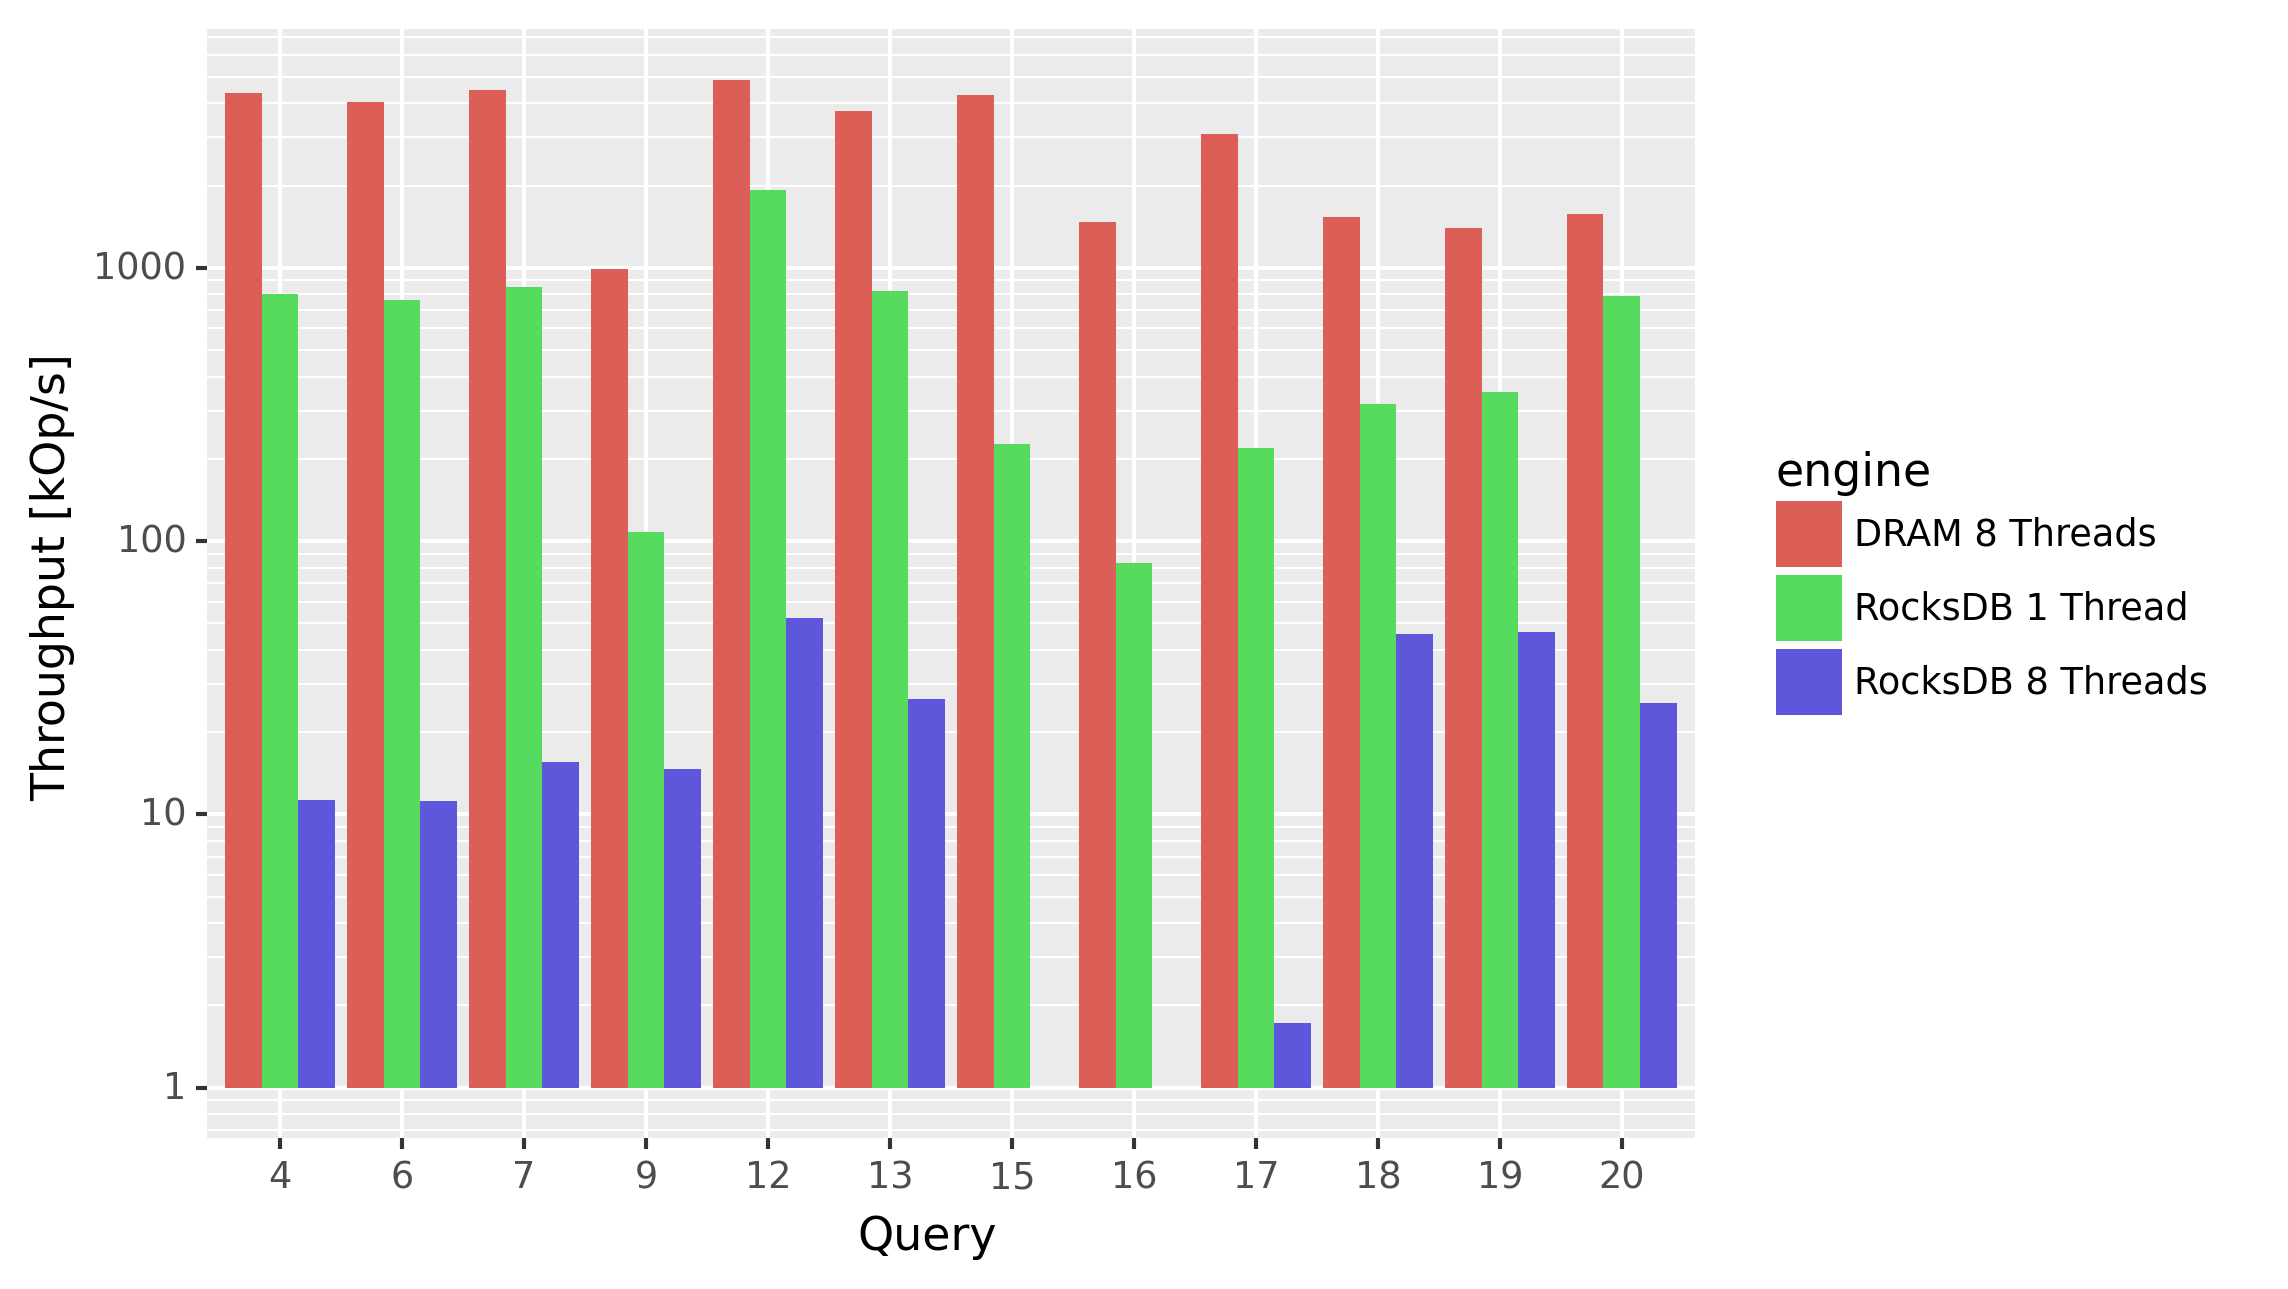
\includegraphics[scale=.43]{graph/rocksdb}
  \caption{Query throughput using RocksDB as a storage layer; higher
    is better.  Note the logarithmic Y axis\label{fig:rocksdb}.}
  \end{center}
\end{figure}

\paragraph{Unable to Leverage Zero-Copy Deserialization.} Besides the
scalability limitations, we also observed significant performance
overheads even when running on a single thread. This was primarily due
to the cost of deserializing keys and values from RocksDB (which
stores data as byte arrays) into the corresponding Rust types.

\paragraph{Overwhelming Configuration Complexity.}

RocksDB offers an overwhelming number of configuration options, making
it nearly impossible for non-experts to ensure optimal settings. The
complexity is so significant that~\cite{thakkar-hotstorage24} resorted
to training a large language model (LLM) to identify good
configurations.

Our attempts did not result in substantial improvements in performance
or scalability. The most effective adjustment was enabling BlobDB,
which increased throughput by approximately 20\%.

\paragraph{Slow Tests Due to Column Families.} Our core engine is tested
using property-based testing, and therefore runs the same unit-tests
with thousands of different inputs.  When these tests required an
index, RocksDB would quickly generate thousands of short-lived column
families (one for each instantiated test).  This caused our test suite
to slow down significantly, extending the total run time from around 2
minutes to approximately 30 minutes.  We traced this issue to a known
performance degradation in RocksDB when creating many column families,
which is unresolved since 2019.

Since we could not find a suitable pre-existing storage system, the
remaining option was to build our own. Building a key-value embedded
database is a substantial endeavor, so we did not make this choice
lightly.

For this purpose, we implemented our own B-tree-like file format. The
traces write each batch that is large enough to an individual file.  Batches
are always created in sorted order, which allowed us to write these
files sequentially without any seeks and with minimal in-memory
buffering.  Because batches are never modified in-place, the file
format and the code that implements it does not need to make
allowances for adding, removing, or modifying data.

Moreover, the implementation of storage extends the in-memory
shared-nothing architecture: each worker thread processes an
independent stream of data, so the storage layer can be per-thread as
well.

\subsubsection{Checkpointing and fault-tolerance}

The state in delay $\zm$ operators is the only piece of information
that needs to be persisted, checkpointed, or migrated to make \dbsp
computations fault-tolerant.  Since \dbsp circuits operate
synchronously in steps, by checkpointing the state between two
execution steps one obtains a consistent snapshot of the circuit's
state.  There is no need for a complicated synchronization protocol.
Since the index data structures are immutable, taking a snapshot can
be done atomically using copy-on-write.  To complete a checkpoint we
just need to ensure that each snapshot is written on secondary
storage.

\subsection{SQL compiler}

We have built a compiler that accepts SQL programs and generates Rust
programs targeting the \dbsp library.  The architecture of the
compiler is shown in Figure~\ref{fig:tools}.  The implementation
follows Algorithm~\ref{algorithm-inc} very closely.  The input of the
algorithm is a non-incremental query plan, produced by a query
planner.  The algorithm produces an incremental plan that is
``similar'' to the input plan.

The compiler front-end, including the parser, validator, and the plan
generator, are based on the Apache Calcite~\cite{begoli-icmd18}
infrastructure.  Because the incrementalization algorithm starts from
a standard, non-incremental query plan, it can reuse in principle any
existing planner.  We rely on Calcite to decorrelate queries into
joins, for optimizing join ordering and performing a host of
traditional optimizations.

A relational algebra query can be implemented by multiple plans, each
with a different data-dependent cost.  Standard query planners use
cost-based heuristics and data statistics to optimize plans.  A
generic IVM planner many not have this luxury, since the plan
sometimes must be generated \emph{before} any data has been fed to the
query.  Nevertheless, all standard query optimization techniques,
perhaps based on historical statistics, can be used to generate the
initial query plan.

The compiler can compile any number of views; each view can depend on
any number of tables or other views.  Given a query $Q$, the compiler
can generate both incremental and non-incremental circuits ($Q$ and
$\inc{Q}$).  The non-incremental circuits are used for validating the
compiler, because they must have the same semantics as a standard
ad-hoc SQL query.

The compiler supports ``standard'' SQL and is mature enough to pass
5+million SQL Logic Tests~\cite{sqllogictest}.
\begin{itemize}
\item \textbf{types:} \code{NULL}s using the standard SQL ternary
  logic, all standard SQL datatypes (including
  \code{DATE}/\code{TIME}/\\\code{TIMESTAMP}), structured and
  semi-structured types, such as arrays, maps, JSON, multisets,
  user-defined functions.
\item \textbf{operators:} \code{SELECT}, \code{WHERE}, \code{FILTER},
  \code{HAVING}, \code{ORDER} \code{BY}, \code{LIMIT},
  \code{DISTINCT}, \code{EXCEPT}, \code{INTERSECT}, \code{UNION},
  \code{GROUP BY}, aggregation, inner and outer \code{JOIN}s,
  \code{PIVOT}, \code{ROLLUP}, \code{CUBE}, temporal \code{ASOF JOIN},
  windows \\ (\code{PARTITION BY ... OVER}), \code{UNNEST}, table
  functions, common table expressions, correlated subqueries, and some
  streaming extensions, like tumbling and hopping windows, etc.
\end{itemize}
The compiler does not yet support recursive queries (although the
runtime does).

SQL has many constructs that may cause runtime exceptions, such as
arithmetic overflows; in a traditional ad-hoc query system these
would surface as queries that terminate with an error.  Currently
these would also cause a running pipeline to fail completely, but this
solution is unacceptable for a platform for long-running computations.
We are exploring alternative solutions, where a runtime crash would
block the pipeline, giving a chance to the operators to remove
incorrect input data that causes issues.

\subsection{Interacting with the outside world}

\begin{figure}[h]
  \begin{center}
  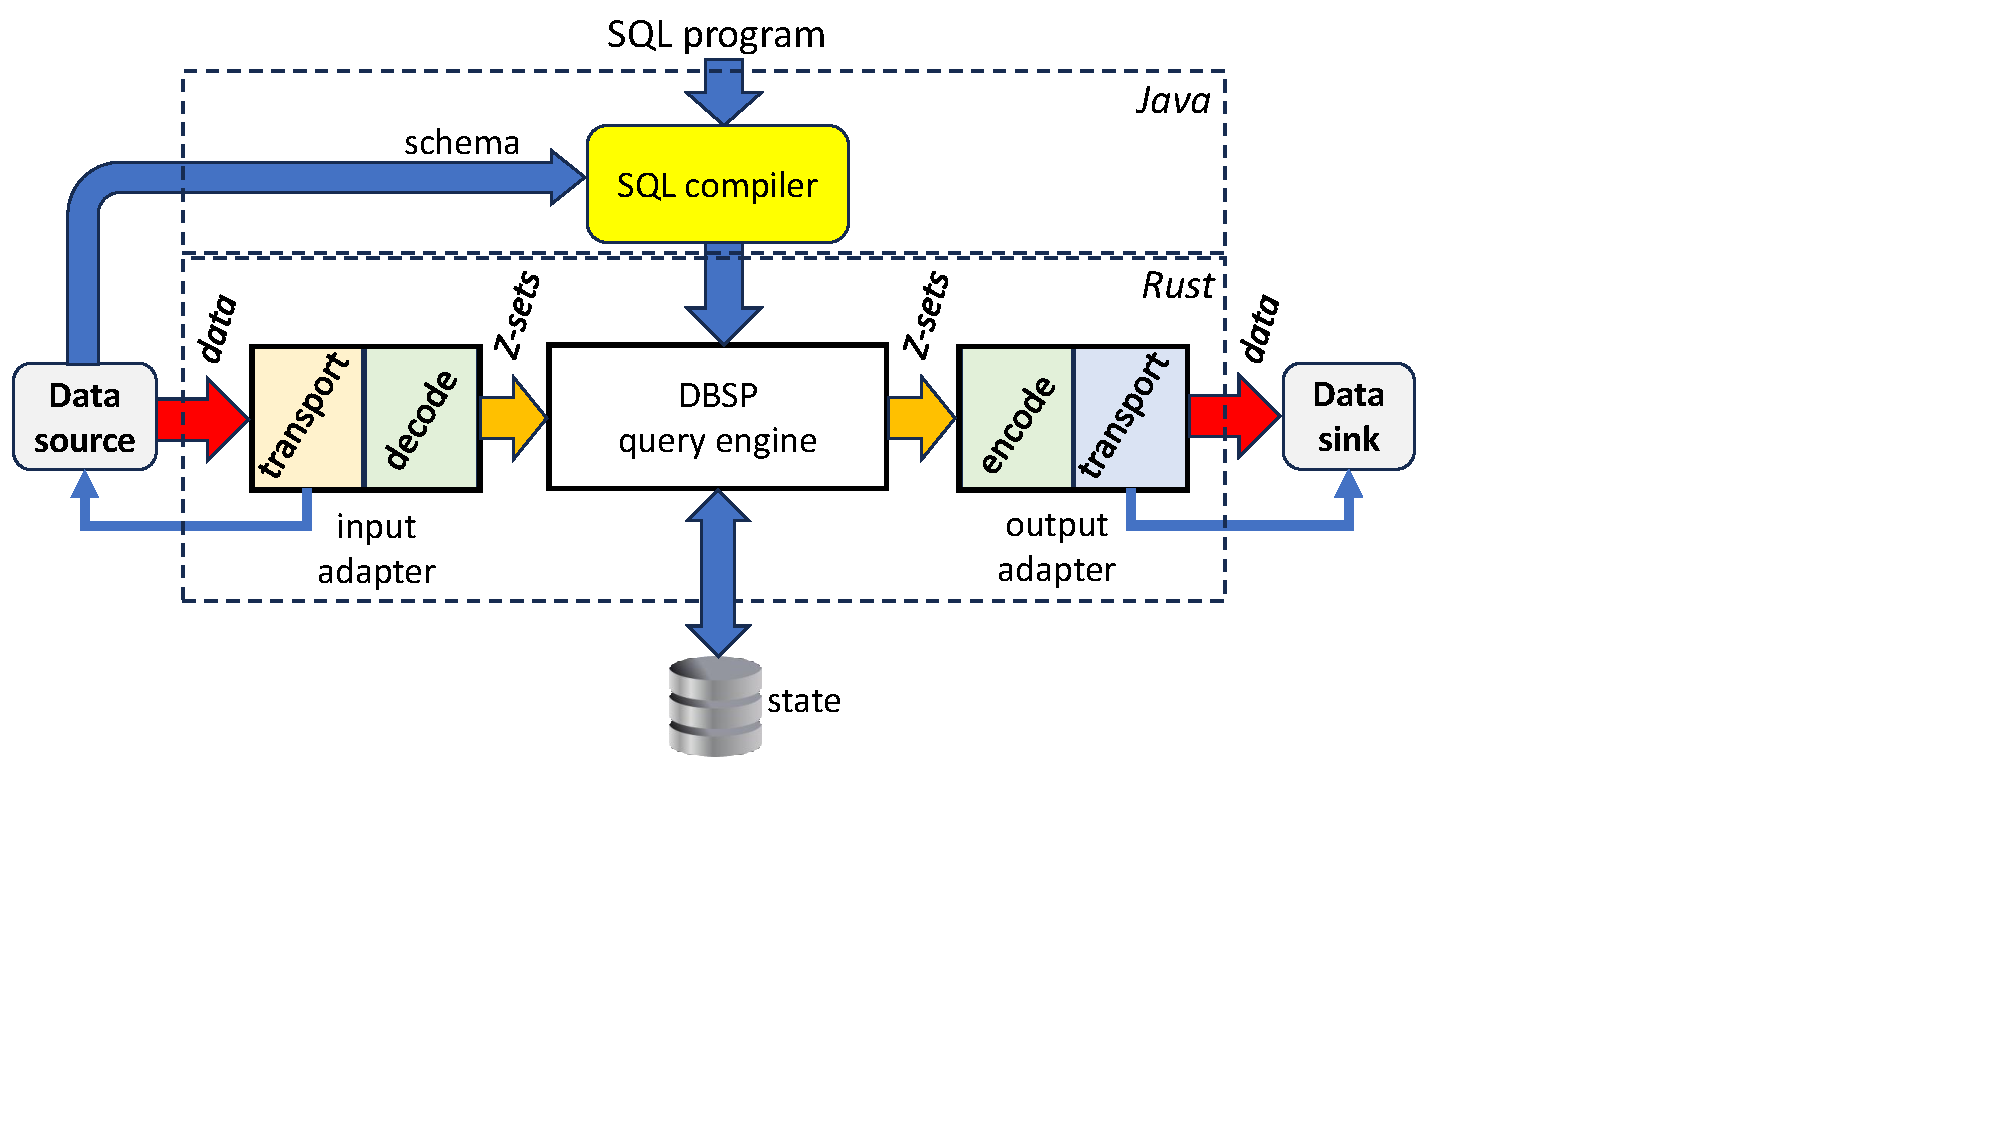
\includegraphics[trim={0 2.2inin 3.7in 0},clip,scale=.33]{adapters.pdf}
  \caption{\label{fig:adapters}Communicating with external data
    sources and sinks.}
  \end{center}
\end{figure}

As noticed many years ago~\cite{labio-vldb00}, database
systems are not designed to interact well with external IVM systems.
We provide a variety of adapters for interacting with external data
sources, both as inputs and outputs (e.g., Kafka~\cite{kreps-netdb11},
Amazon S3~\cite{palankar-dadc08}, Google Pub/Sub~\cite{pubsub},
DataFrames~\cite{pandas12}, Databricks Delta
Lake~\cite{armbrust-vldb20}, database CDC streams via
Debezium~\cite{debezium}, http, etc.), and using many data formats
(CSV, JSON, Avro, Parquet, etc.).  Figure~\ref{fig:adapters} shows how
a circuit uses adapters to communicate with the outside world.  The
input adapters receive data from external sources, buffer it, convert
it into \zrs, and feed it to the circuits.  The output adapters
receive data from the circuit outputs in the form of \zrs, and send it
to a downstream consumer in a suitable format.

\begin{figure}[h]
  \begin{center}
  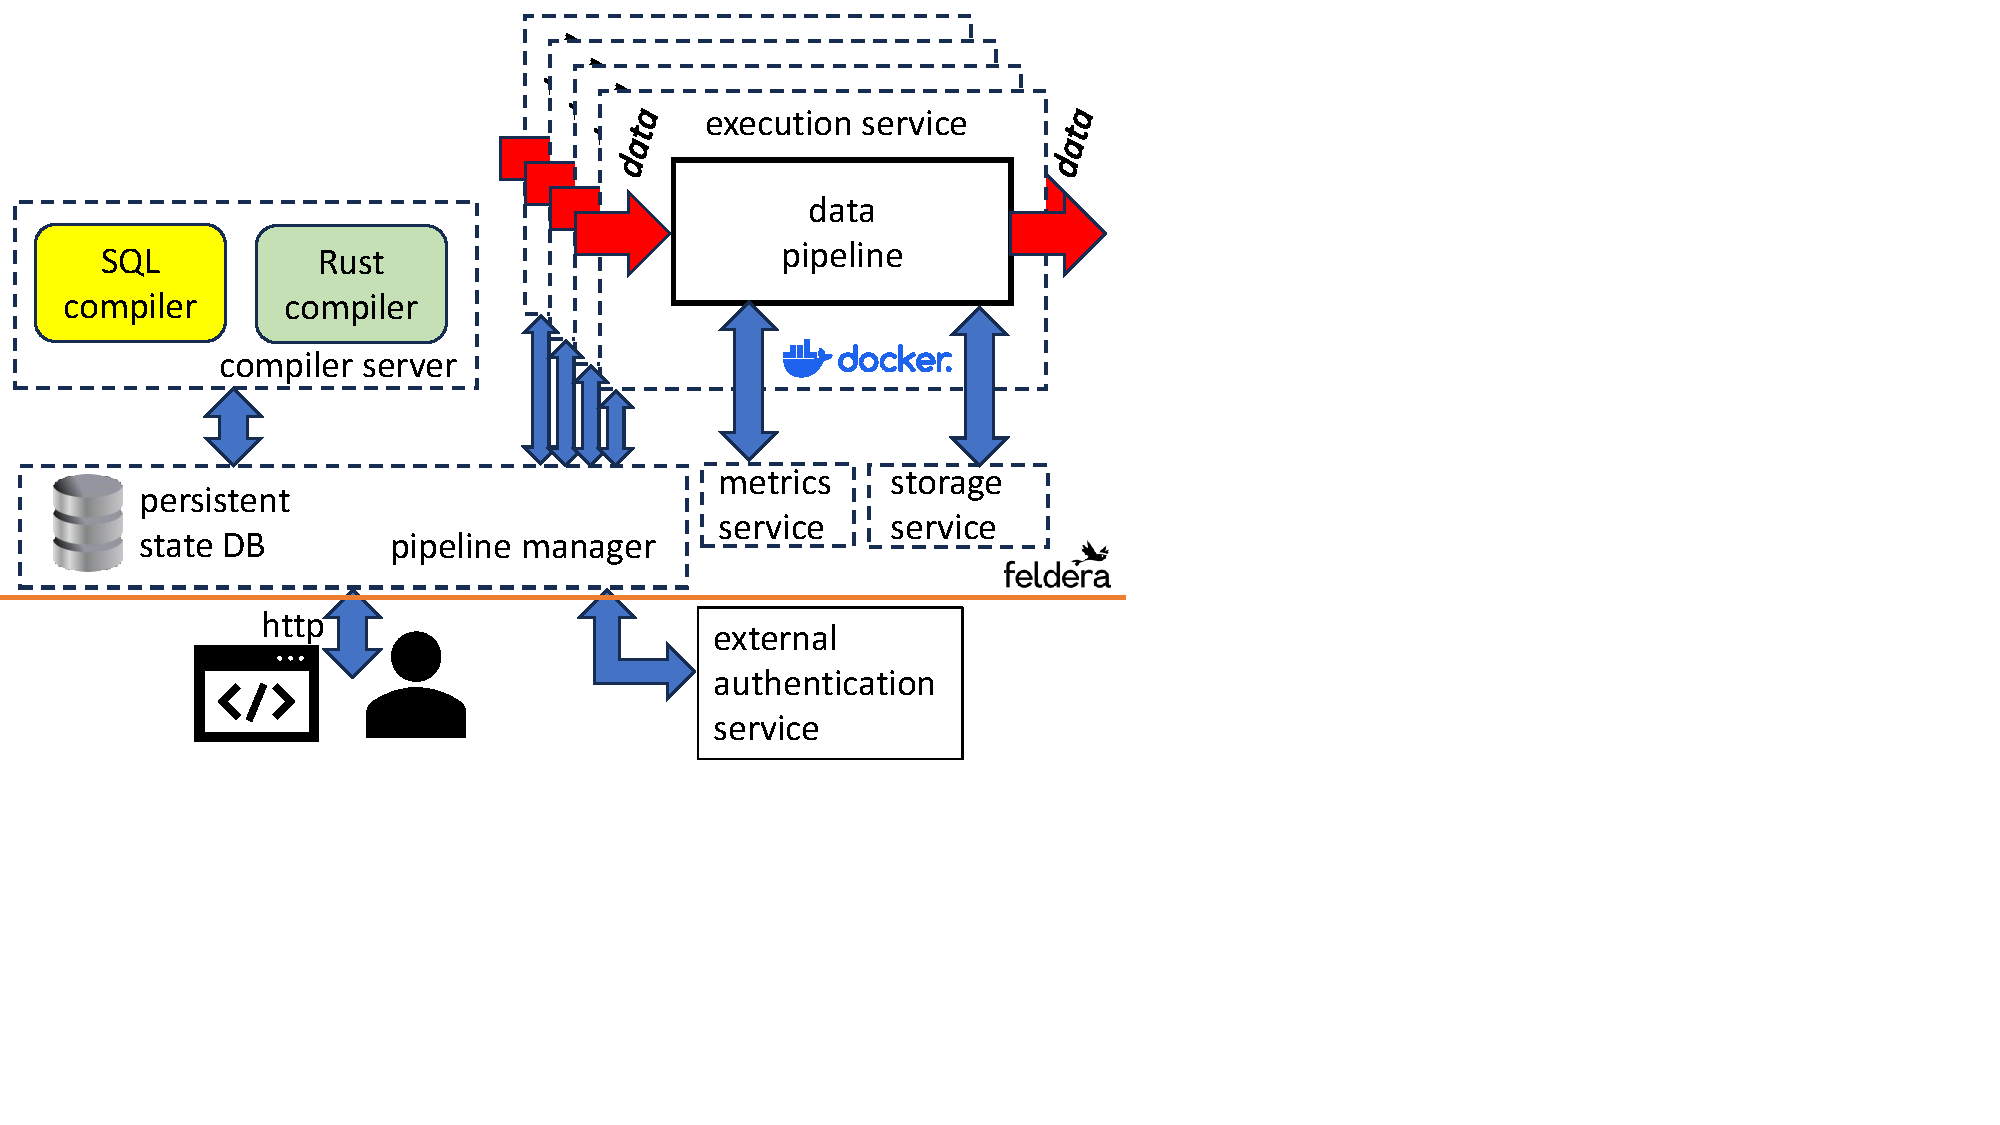
\includegraphics[trim={0 2.4in 4.3in 0},clip,scale=.44]{services.pdf}
  \caption{\label{fig:service}Feldera Service architecture.}
  \end{center}
\end{figure}

Feldera as a company offers IVM as a service.  The service-oriented
architecture of the company's cloud offering is shown in
Figure~\ref{fig:service}.  The pipeline manager is the centralized
control plan, which is responsible for managing the entire life-cycle
of the IVM programs.  These programs are deployed as \emph{pipelines}
that run in isolated Docker containers.

